\documentclass[../main]{subfiles}
\begin{document}


\chapter{Onda Sinusoidal}

\img{images/10/sinusoide.jpg}{Osciloscopio digital.}

\info{Sinusoide}{Se denomina sinusoide a la curva que representa gráficamente la función seno y también a dicha función en sí Es una curva que describe una oscilación repetitiva y suave.
Su forma más básica en función del tiempo (t) es:
\begin{equation}
y(t)= a \sen(\omega t+\varphi)    
\end{equation}

}
La sinusoide puede ser descrita por las siguientes expresiones matemáticas:


\begin{center}
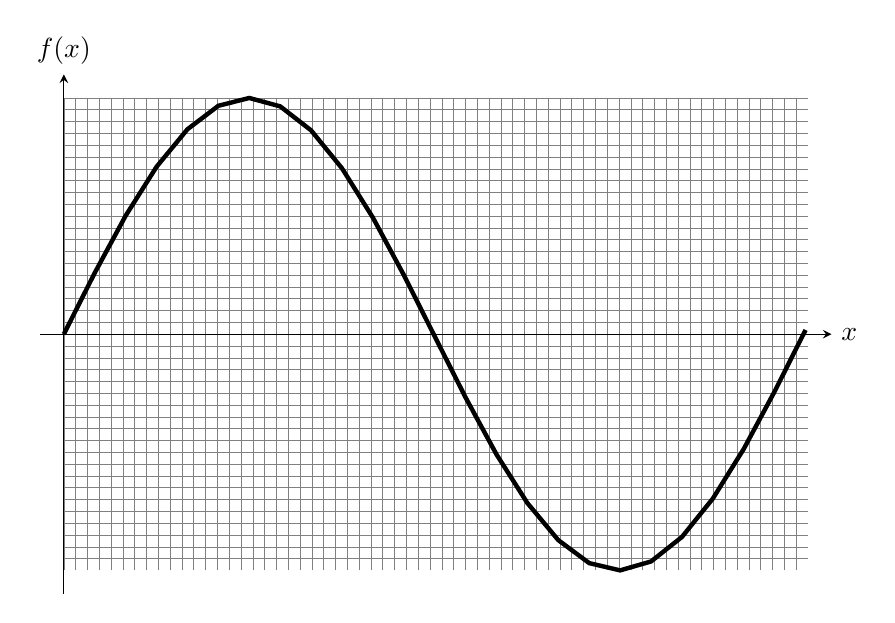
\begin{tikzpicture}[domain=0:6.28,scale=1.5]
    \draw[very thin,color=gray,step=0.1] (0,-2) grid (6.3,2);
    \draw (-0.2,0) -- (6.5,0) [-stealth] node[right] {$x$};
    \draw (0,-2.2) -- (0,2.2) [-stealth] node[above] {$f(x)$};
    \draw[ultra thick,color=black] plot (\x,{2*sin(2*3.1415*\x*9.15)});
 \end{tikzpicture}
\end{center}

$y(x)=a\ {\rm {sen}}\left(\omega x+\varphi \right) ;\quad y(t)=a\ {\rm {sen}}\left(2 \pi f t+\varphi \right) ;\quad y(x)=a\ {\rm {sen}}\left(\dfrac{2 \pi}{T} x+\varphi \right)$

\subsection{Impedancia}

\info{Reactancia capacitiva $X_C$ e inductiva $X_L$}{
Reactancia Inductiva
\begin{equation}
    X_L= \omega L
\end{equation}
Reactancia Capacitiva
\begin{equation}
    X_C= \dfrac{1}{\omega C}
\end{equation}

como $\omega=2 \pi f$
Reactancia Inductiva
\begin{equation}
    X_L= 2 \pi f L
\end{equation}
Reactancia Capacitiva
\begin{equation}
    X_C= \dfrac{1}{2 \pi f C}
\end{equation}
}


\info{Impedancia eléctrica $Z$}{

\begin{equation}
    Z= \sqrt{R^2+(X_L-X_C)^2}
\end{equation}
}


\actividad{Resolver las siguientes problemas.}
\begin{enumerate}
    \item Dibujar una onda sinusoidal a través de el circulo generador ($r=5cm$).
    \begin{enumerate}
        \item Calcular el área bajo la curva y su valor medio.
        \item Calcular el valor eficáz como la raiz cuadrada del del promedio de los cuadrados de los valores.
        \item Graficar los valores medio y eficaz.
        
    \end{enumerate}
 \item - Una onda de corriente alterna senoidal tiene por expresión analítica: $i(t)=6 \sen(6280 t)$
    \begin{enumerate}
        \item Calcular el valor medio.
        \item Calcular la frecuencia y el período.
        \item Obtener el valor instantáneo que toma la onda transcurridos 0.02 ms.
        \item Calcular el valor eficaz.
        \item El valor que toma la onda para un ángulo $\alpha = 120^\circ$.
    \end{enumerate}

\item Una onda de corriente alterna senoidal tiene por expresión analítica:
$i(t)=12\sen(\omega t)$. Calcular el valor medio y eficáz.
\item Una onda senoidal de $f=60Hz$ de frecuencia tiene un valor eficaz de $V_{ef}=125V$. Calcular la duración del periodo $T$ y la expresión que define la onda de tensión instantánea $i(t)$.
\item Una resistencia de valor $R=100\Omega$ se somete a una tensión alterna de valor
$u(t)=5\sen(3140 t)$
Calcular:
\begin{enumerate}
    \item La intensidad que absorbe.
    \item La energía térmica que se transforma al cabo de dos horas de funcionamiento.
\end{enumerate}
\item Una impedancia tiene una resistencia de $R=30\Omega$ y una reactancia inductiva de $X_L=40\Omega$. Se
somete a una tensión alterna de 24 V - 50 Hz. Calcular:
\begin{enumerate}
    \item Su impedancia $Z$.
\item La intensidad que absorbe $I$.
\item Las potencias:activa $P$,reactiva $Q$ y aparente $S$.
 
\end{enumerate}
\item Una bobina de reactancia está formada por un hilo de cobre de $S=0,5mm^2$ de sección y $N=1500$
espiras de $l=0,1m$ de longitud media cada vuelta. Se somete a una corriente alterna de $f=1KHz$ de
frecuencia y da una inductancia $L=400mH$. Calcular su impedancia $Z$.
\item Una resistencia de $R=1000\Omega$ se conecta en serie con un condensador de $C=2,2\mu F$ y el conjunto
se somete a una tensión alterna de $V=6V ;\quad f=50Hz$.
\begin{enumerate}
\item Calcular la impedancia $Z$.
\item La intensidad que absorbe $I$.
\item El factor de potencia. $\cos(\varphi)$
\item Las potencias  activa $P$, reactiva $Q$ y aparente $S$. Representarlas vectorialmente.
\end{enumerate}


\end{enumerate}
\newpage
\end{document}